% Final defense deck: 19 pages, CN+EN ISSCC/VLSI minimalist theme
% Build: python3 make_data.py && latexmk -xelatex main.tex
% Every metric is a macro generated into data/ by make_data.py from verified repository records.
\documentclass[10pt,aspectratio=169,hyperref={colorlinks,urlcolor=steel,linkcolor=}]{beamer}
\usepackage{PekingU}
\setbeamertemplate{headline}{}
\makeatletter\AtBeginDocument{\global\pku@headheight=0pt}\makeatother
\setbeamertemplate{background canvas}{\color{white}\rule{\paperwidth}{\paperheight}}
\usefonttheme{professionalfonts}
\usepackage{fontspec}
\usepackage{xeCJK}
\xeCJKsetup{CJKmath=true}
% CJK: Microsoft YaHei (TrueType collection) via fontconfig discovery; PingFang SC on macOS; Noto Sans CJK SC on Linux. Never the ctex default serif.
\IfFontExistsTF{Microsoft YaHei}{%
  \setCJKmainfont{Microsoft YaHei}[BoldFont=Microsoft YaHei Bold,ItalicFont=Microsoft YaHei]%
  \setCJKsansfont{Microsoft YaHei}[BoldFont=Microsoft YaHei Bold,ItalicFont=Microsoft YaHei]%
  \setCJKmonofont{Microsoft YaHei}[BoldFont=Microsoft YaHei Bold,ItalicFont=Microsoft YaHei]%
}{%
  \IfFontExistsTF{PingFang SC}{%
    \setCJKmainfont{PingFang SC}\setCJKsansfont{PingFang SC}\setCJKmonofont{PingFang SC}%
  }{%
    \setCJKmainfont{Noto Sans CJK SC}\setCJKsansfont{Noto Sans CJK SC}\setCJKmonofont{Noto Sans CJK SC}%
  }%
}
\renewcommand{\CJKfamilydefault}{\CJKsfdefault}

% Strictly TrueType (.ttf) sans-serif & monospace fonts for universal pdf.js rendering
\IfFontExistsTF{Segoe UI}{%
  \setsansfont{Segoe UI}%
}{%
  \IfFontExistsTF{Helvetica Neue}{%
    \setsansfont{Helvetica Neue}%
  }{%
    \setsansfont{LiberationSans-Regular.ttf}[
      Path=/usr/share/fonts/truetype/liberation/,
      BoldFont=LiberationSans-Bold.ttf,
      ItalicFont=LiberationSans-Italic.ttf,
      BoldItalicFont=LiberationSans-BoldItalic.ttf
    ]%
  }%
}
\IfFontExistsTF{Consolas}{%
  \setmonofont{Consolas}[Scale=0.92]%
}{%
  \IfFontExistsTF{Menlo}{%
    \setmonofont{Menlo}[Scale=0.92]%
  }{%
    \setmonofont{LiberationMono-Regular.ttf}[
      Path=/usr/share/fonts/truetype/liberation/,
      BoldFont=LiberationMono-Bold.ttf,
      Scale=0.92
    ]%
  }%
}
\renewcommand{\familydefault}{\sfdefault}

\usepackage{amsmath,amssymb,xcolor,booktabs,graphicx,ragged2e,parskip,tabularx,array,multirow,colortbl}
\usepackage{tikz}
\usetikzlibrary{positioning,arrows.meta,calc}
\usepackage{pgfplots}
\pgfplotsset{compat=1.18}
\apptocmd{\frame}{}{\justifying}{}

\input{data/numbers.tex}
\makeatletter\newcommand{\tabinput}[1]{\@@input #1 }\makeatother

% ---------- ISSCC / VLSI Restrained Minimalist Palette ----------
\definecolor{peking}{HTML}{8B0012}     % Primary Accent: PKU Crimson
\definecolor{ink}{HTML}{1E293B}        % Primary Ink: Deep Charcoal
\definecolor{muted}{HTML}{64748B}      % Secondary Text / Captions
\definecolor{hair}{HTML}{D8DEE6}       % Hairline Rules & Borders
\definecolor{surf}{HTML}{F6F7F9}       % Neutral Light Surface
\definecolor{steel}{HTML}{1D4E89}      % Secondary Chart Accent: Deep Steel Blue
\definecolor{passink}{HTML}{15803D}    % Subtle Semantic Pass
\definecolor{warnink}{HTML}{B45309}    % Subtle Semantic Attention

\setbeamercolor{normal text}{fg=ink,bg=white}
\setbeamercolor{frametitle}{fg=peking,bg=white}
\setbeamercolor{structure}{fg=peking}
\setbeamercolor{footline}{bg=peking,fg=white}
\setbeamercolor{title}{bg=peking,fg=white}
\setbeamerfont{frametitle}{series=\bfseries,size=\large}
\setbeamerfont{section in toc}{series=\bfseries,size=\normalsize}
\setbeamerfont{itemize/enumerate body}{size=\scriptsize}
\setbeamerfont{itemize/enumerate subbody}{size=\scriptsize}
\setbeamertemplate{itemize item}{\raisebox{0.18ex}{\tikz\fill[peking] (0,0) rectangle (3pt,3pt);}}
\setbeamertemplate{itemize subitem}{\raisebox{0.18ex}{\tikz\draw[muted,line width=0.6pt] (0,0) circle (1.3pt);}}
\setbeamertemplate{enumerate item}{\textbf{\color{peking}\insertenumlabel.}}

\title[先进芯片全栈设计与协同优化]{先进芯片全栈设计与协同优化\\[4pt]{\large Full-Stack Chip Design \& Hardware-Software Co-Optimization}}
\subtitle{RTL 微架构 · 编译器与主机传输 · \NSealInt{} µm MMMC 签核 · \NSysClk{} MHz EGo1 实板}
\author[]{Ruijun He \quad Guoyi Zhang \quad Zhiyuan Zhao \quad Muyang Cheng}
\institute{Peking University}
\date{November 2026}

% ---------- Clean Helpers ----------
\newcommand{\hl}[1]{\textcolor{peking}{\textbf{#1}}}
\newcommand{\snote}[1]{{\scriptsize\color{muted}#1\par}}
\newcommand{\ok}{\tikz[baseline=-0.1ex]\draw[passink,line width=1.15pt,line cap=round,line join=round] (0,0.34ex) -- (0.36ex,-0.02ex) -- (0.98ex,0.82ex);}
\newcommand{\pending}{\textcolor{warnink}{\textbf{–}}}

% Crisp Left-Bar Callout (Zero full-sided colored boxes)
\newcommand{\callout}[2][peking]{%
  \noindent\begin{tikzpicture}
    \node[anchor=north west, fill=surf, text=ink, inner xsep=8pt, inner ysep=6pt,
          text width=\dimexpr\linewidth-16pt\relax, align=left, font=\scriptsize] (box) {#2};
    \fill[#1] (box.north west) rectangle ([xshift=2.4pt]box.south west);
  \end{tikzpicture}%
}

\tikzset{
  issccbox/.style={draw=ink!80, line width=0.75pt, rounded corners=1.5pt, fill=white,
                   align=center, font=\scriptsize, inner sep=4pt, minimum height=0.95cm, text width=#1},
  issccbox/.default=1.8cm,
  issccarr/.style={-{Stealth[length=4.5pt,width=3.2pt]}, line width=0.75pt, draw=ink!80},
  issccnote/.style={font=\tiny, text=ink!85, inner sep=1pt, outer sep=2pt},
}

\pgfplotsset{
  issccbar/.style={
    font=\scriptsize,
    axis lines*=left,
    axis line style={ink!60, line width=0.6pt},
    tick style={ink!50},
    grid style={hair, line width=0.4pt},
    tick label style={font=\scriptsize, text=ink},
    xticklabel={\pgfmathprintnumber[assume math mode=true]{\tick}},
    yticklabel={\pgfmathprintnumber[assume math mode=true]{\tick}},
    label style={font=\scriptsize, text=ink},
    legend style={font=\scriptsize, draw=none, fill=none},
    /pgf/number format/assume math mode=true,
  },
}

\setlength{\tabcolsep}{4pt}
\renewcommand{\arraystretch}{1.18}


\pgfplotsset{
  isscclab/.style={
    font=\scriptsize, axis lines*=left, axis line style={ink!60, line width=0.6pt},
    tick style={ink!50}, grid style={hair, line width=0.4pt},
    tick label style={font=\tiny, text=ink}, label style={font=\tiny, text=ink},
    legend style={font=\tiny, draw=none, fill=none}, title style={font=\scriptsize\bfseries, text=ink},
  },
}
\definecolor{cA}{HTML}{8B0012}\definecolor{cB}{HTML}{1D4E89}\definecolor{cC}{HTML}{15803D}
\definecolor{cD}{HTML}{B45309}\definecolor{cE}{HTML}{6D28D9}\definecolor{cF}{HTML}{0E7490}\definecolor{cG}{HTML}{64748B}

% Card: thin top rule + kicker + heading
\newcommand{\card}[3][ink]{{\color{#1}\rule{\linewidth}{1.4pt}}\par\vspace{3pt}{\tiny\bfseries\color{#1!90!muted} #2}\par\vspace{1pt}{\footnotesize\bfseries\color{ink} #3}\par\vspace{3pt}}
\newcommand{\bignum}[2]{{\large\bfseries\color{peking}#1}\,{\scriptsize\color{muted}#2}}
\newcommand{\tsub}[1]{\texttt{#1}}

\begin{document}

% ===================================================================== 01 Cover
{\setbeamertemplate{logo}{}
\begin{frame}
  \titlepage
  \vspace{-6pt}
  \begin{center}
\includegraphics[width=0.19\linewidth]{Figures/PKU-emblem-names.png}\end{center}
\end{frame}}

% ===================================================================== 02 Scorecard
\begin{frame}{全栈核心指标总览 · Executive Full-Stack KPI Scorecard}
  \begin{columns}[T,onlytextwidth]
    \column{0.235\textwidth}
      \card[peking]{01 · RTL CO-OPT}{RTL 微架构协同优化}
      \bignum{\NCols×\NCols}{INT4 MAC Array}\par\vspace{3pt}
      \begin{itemize}\setlength{\itemsep}{1pt}
        \item 写回流水 + 寄存式 Element ALU 捕获
        \item FPGA \tsub{use\_dsp} DSP48E1 MAC
        \item 4-state 复位卫生：\NRetTwoResetRegs{} 个 \tsub{ret2} 控制寄存器 + \NWriteDepth{} 级写队列
        \item RTL 审计 \NAuditExact/\NAuditFrames{} 帧 0-bit
      \end{itemize}
    \column{0.235\textwidth}
      \card[steel]{02 · COMPILER \& HOST}{统一编译器与主机传输}
      \bignum{\NRTwBaseHostOps{}→\NRTwHwHostOps}{R20 Host Ops}\par\vspace{3pt}
      \begin{itemize}\setlength{\itemsep}{1pt}
        \item ResNet-18 Tile \NREiBaseTiles{}→\NREiHwTiles{}（−\NREiTilePct\%）
        \item \tsub{OP\_ADD=\NOpAdd} 残差硬件化，Conv+MaxPool 融合
        \item IR/I-O 几何驻留缓存，\NWriteChunk{}-word 写块
        \item FT232H FIFO 修复：读块 \NReadChunk{} word = \NReadChunkBytes{} B
      \end{itemize}
    \column{0.235\textwidth}
      \card[peking]{03 · ASIC SIGNOFF}{\NSealInt{} µm 物理签核}
      \bignum{\NMmmcViol}{4-Corner MMMC 违例}\par\vspace{3pt}
      \begin{itemize}\setlength{\itemsep}{1pt}
        \item \NAsicClk{} MHz，\tsub{ss125} Setup +\NSSSetup{} ns，±\NRcPct\% RC \NRcViol{} 违例
        \item STA +\NStaSetup/+\NStaHold{} ns，LEC \NLecPass
        \item 双角 SDF \NSdfJtag{}-JTAG \NSdfPass
        \item DRC \NDrcBlocking{} 阻断 · nmLVS \NLvsStatus{} · ANT/WB 0
      \end{itemize}
    \column{0.235\textwidth}
      \card[steel]{04 · LIVE FPGA}{\NSysClk{} MHz EGo1 实板}
      \bignum{\NZooExact/\NZooRuns}{zoo 推理 0-bit}\par\vspace{3pt}
      \begin{itemize}\setlength{\itemsep}{1pt}
        \item \NZooModels{} 模型 × \NTckCount{} 档 TCK（\NTckMin–\NTckMax{} MHz）
        \item 六场景 \NSceneExact/\NSceneFrames{} 代表帧一致
        \item ResNet-20 \NRTwSamples/\NRTwSamples{} 帧 bit-exact
        \item ResNet-18 \NREiSamples{} 帧实板 bit-exact
      \end{itemize}
  \end{columns}\par\vspace{8pt}
  \callout[peking]{\textbf{主线}：同一份 RTL（\tsub{\NAsicCommit}）同时驱动 TSMC 180 nm \NSealInt{} µm 签核与 \NSysClk{} MHz EGo1 实板；编译器把残差加法下沉到硬件（\tsub{OP\_ADD}），主机传输修复 FT232H 死锁后，ResNet-20/18 在 \NSramKB{} KB 片上 SRAM 上实板 \hl{0-bit 精确}。瓶颈已定位在 USB/JTAG 传输（ResNet-20 占墙钟 \hl{\NRTwJtagPct\%}）。}
\end{frame}

% ===================================================================== 03 Architecture
\begin{frame}{SoC 与可编程 NPU 架构 · SoC \& Programmable NPU Architecture}
  \begin{columns}[T,onlytextwidth]
    \column{0.60\textwidth}
    \centering
    \begin{tikzpicture}[node distance=0.42cm and 0.42cm, font=\scriptsize]
      \node[issccbox=1.55cm] (host) {\textbf{Host PC}\\Compiler +\\Runtime};
      \node[issccbox=1.35cm, right=of host] (ftdi) {FT232H\\MPSSE\\USB→JTAG};
      \node[issccbox=1.55cm, right=of ftdi, fill=surf] (tap) {\textbf{JTAG TAP}\\\NJtagPacketBits-bit packet\\TCK domain};
      \node[issccbox=1.55cm, right=0.55cm of tap, draw=peking, line width=1pt] (cdc) {\textbf{Mailbox CDC}\\\NSyncStages-FF toggle\\req/ack sync};
      \node[issccbox=2.3cm, below=0.62cm of cdc.south east, anchor=north east] (ctl) {\textbf{Command Controller}\\sys\_clk domain};
      \node[issccbox=3.1cm, below=0.5cm of ctl, draw=peking, line width=1pt, fill=surf, minimum height=1.25cm] (npu) {\textbf{\tsub{npu\_program\_core}}\\\NCols×\NRows{} INT4 Systolic MAC\\Requant · Element ALU (Add/Pool)\\≤\NMaxOps{} ops, K≤\NMaxK};
      \node[issccbox=3.6cm, left=0.5cm of npu, draw=steel, line width=1pt, minimum height=1.25cm] (sram) {\textbf{Unified \NSramKB{} KB SRAM}\\\NMacroCount× \tsub{\NSramMacro}\\Activation + Model Tail\\(\NActBytes{} B shared)};
      \draw[issccarr] (host) -- (ftdi);
      \draw[issccarr] (ftdi) -- node[issccnote,above]{TCK} (tap);
      \draw[issccarr] (tap) -- (cdc);
      \draw[issccarr] (cdc.south -| ctl.north) -- (ctl.north);
      \draw[issccarr] (ctl) -- node[issccnote,right]{desc./start} (npu);
      \draw[issccarr, steel, <->] (npu) -- node[issccnote,above]{rd/wr} (sram);
      \draw[issccarr, steel, <->] (ctl.west) -| node[issccnote,above, pos=0.25]{host load/readback} (sram.north);
      \node[issccnote, text=muted, anchor=south] at ($(cdc.north)+(0,0.08)$) {TCK $\rightleftarrows$ SYS};
    \end{tikzpicture}
    \column{0.37\textwidth}
    {\small\textbf{ABI \NAbi{} 统一 SRAM 契约}}
    \begin{itemize}\setlength{\itemsep}{1pt}
      \item \NMacroCount{} 个 \NSramMacroKB{} KB 单口宏组成 \NSramBytes{} B 统一地址空间：激活与模型尾部共享，编译器按同一预算切块。
      \item 主机只通过 JTAG 邮箱访问：\NJtagPacketBits-bit 命令包，Burst IR 每次扫描传 1 个 32-bit 字。
    \end{itemize}\par\vspace{3pt}
    {\small\textbf{跨时钟域}}
    \begin{itemize}\setlength{\itemsep}{1pt}
      \item 请求/应答 toggle 经 \NSyncStages-FF \tsub{ASYNC\_REG} 同步链；复位异步置位、两域独立同步释放。
      \item Burst 读最坏往返 \NBurstSysCycles{} 个 sys\_clk，主机据此插入 ≥\NIdleTckMin{} 个空闲 TCK。
    \end{itemize}\par\vspace{3pt}
    {\small\textbf{实现目标}}
    \begin{itemize}\setlength{\itemsep}{1pt}
      \item ASIC：TSMC 180 nm，\NAsicClk{} MHz（\NAsicPeriod{} ns）。
      \item FPGA：EGo1 XC7A35T，\NSysClk{} MHz，同步 BRAM。
    \end{itemize}
  \end{columns}
\end{frame}

% ===================================================================== 04 RTL co-opt
\begin{frame}{硬件微架构协同优化 · RTL Microarchitecture Co-Opt}
  \begin{columns}[T,onlytextwidth]
    \column{0.315\textwidth}
      \card[peking]{PR \#28 · TIMING}{结果写回流水化}
      \begin{itemize}\setlength{\itemsep}{1pt}
        \item 原路径：psum 归约 → +bias → 池化比较 → \tsub{results} 写入在同一拍完成。
        \item 新增 \tsub{ret2} 级：先锁存 \NCols×\NPsumBits-bit 归约结果（\NRetTwoFlops{} 个 FF），下一拍再加 bias 并比较。
        \item \tsub{compute\_drained} 额外等待 \tsub{!ret2\_valid}，保证排空语义不变。
      \end{itemize}
    \column{0.315\textwidth}
      \card[steel]{PR \#28 · ALU / FPGA}{寄存式 Element ALU 与 DSP}
      \begin{itemize}\setlength{\itemsep}{1pt}
        \item SRAM 读数据先存入 \tsub{e\_data\_q}（新状态 \tsub{estate=4}），Add/Pool/AvgPool 从寄存器取数，切断 SRAM→ALU→\tsub{results} 长组合路径。
        \item \tsub{CHIPDESIGN\_FPGA\_MEM} 下 MAC 标注 \tsub{use\_dsp="yes"}，推断 DSP48E1；ASIC 仍为标准单元（\tsub{"no"}）。
      \end{itemize}
    \column{0.315\textwidth}
      \card[peking]{PR \#30 · 4-STATE}{复位卫生（\tsub{npu\_program\_core.sv}）}
      \begin{itemize}\setlength{\itemsep}{1pt}
        \item \tsub{begin\_tile} 清零 \tsub{ret2\_slot} / \tsub{tap\_first} / \tsub{tap\_last} / \tsub{pos\_addr}。
        \item 复位时清零 \NWriteDepth{} 级写合并队列的 \tsub{write\_addr/mask/data}。
        \item 仅改动复位/清零赋值，不改数据通路；签核网表即含此修复（\tsub{\NAsicCommit}）。
      \end{itemize}
  \end{columns}\par\vspace{6pt}
  \callout[warnink]{\textbf{为何修复了 \tsub{ss125\_max} 的 \texttt{X} 泄漏}：两态 RTL 仿真中未复位寄存器读作 0，问题不可见；门级 SDF 四态仿真里它们上电为 \texttt{X}。写合并队列与 \tsub{ret2} 控制位的 \texttt{X} 经写路径进入 Activation Store，污染直接映射缓存标签 \tsub{cache\_tag[6]}（共 \NCacheTagFlops{} 个 tag FF），使命中判断与读回数据变为 \texttt{X}。补上复位后，\tsub{ss125\_max} 与 \tsub{ffm40\_min} 双角 \NSdfJtag{} 条 JTAG 命令全部 \NSdfPass。}
  \par\vspace{3pt}\snote{行为级 RTL 与 FPGA 结果不受影响：两者本就逐位一致；该修复只消除门级四态仿真中的悲观 \texttt{X} 传播。}
\end{frame}

% ===================================================================== 05 Compiler
\begin{frame}{图编译器、SRAM 切块与算子融合 · Compiler \& Fusion}
  \begin{columns}[T,onlytextwidth]
    \column{0.50\textwidth}
    \centering
    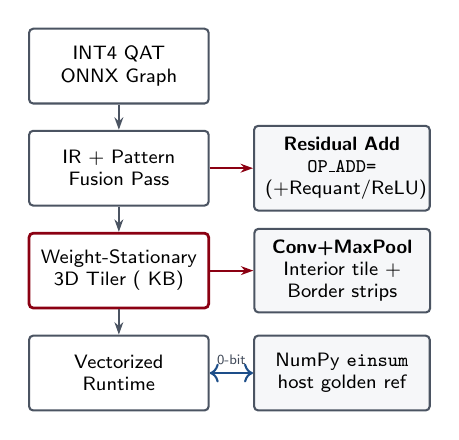
\begin{tikzpicture}[node distance=0.32cm, font=\scriptsize]
      \node[issccbox=2.0cm] (onnx) {INT4 QAT\\ONNX Graph};
      \node[issccbox=2.0cm, below=of onnx] (ir) {IR + Pattern\\Fusion Pass};
      \node[issccbox=2.0cm, below=of ir, draw=peking, line width=1pt] (tile) {Weight-Stationary\\3D Tiler (\NSramKB{} KB)};
      \node[issccbox=2.0cm, below=of tile] (rt) {Vectorized\\Runtime};
      \node[issccbox=1.95cm, right=0.55cm of ir, fill=surf] (add) {\textbf{Residual Add}\\\tsub{OP\_ADD=\NOpAdd}\\(+Requant/ReLU)};
      \node[issccbox=1.95cm, right=0.55cm of tile, fill=surf] (pool) {\textbf{Conv+MaxPool}\\Interior tile +\\Border strips};
      \node[issccbox=1.95cm, right=0.55cm of rt, fill=surf] (np) {NumPy \tsub{einsum}\\host golden ref};
      \foreach \a/\b in {onnx/ir, ir/tile, tile/rt} \draw[issccarr] (\a) -- (\b);
      \draw[issccarr, peking] (ir) -- (add);
      \draw[issccarr, peking] (tile) -- (pool);
      \draw[issccarr, steel, <->] (rt) -- node[issccnote,above]{0-bit} (np);
    \end{tikzpicture}
    \column{0.47\textwidth}
    {\small\textbf{硬件残差卸载（\tsub{OP\_ADD = \NOpAdd}）}}
    \begin{itemize}\setlength{\itemsep}{1pt}
      \item 单描述符 Add 包：in1 位于偏移 0，in2 位于 \tsub{align4(in1\_bytes)}；按空间与通道切块。
      \item NPU 计算 $w_a a + w_b b$ 并在片上 Requant/ReLU，主机后处理算子归零（ResNet-20：\NRTwBaseHostOps{} → \NRTwHwHostOps）。
    \end{itemize}\par\vspace{3pt}
    {\small\textbf{Conv+MaxPool 融合与边界/内部 Halo 拆分}}
    \begin{itemize}\setlength{\itemsep}{1pt}
      \item 池化输出分为无 padding 的内部区与 padding 边界条：内部区直接以 Conv→Requant→MaxPool 单程序执行。
      \item 边界条拆为 Conv 条带 + 带 padding 的 Pool 小块，保证与参考逐位一致。
    \end{itemize}\par\vspace{3pt}
    {\small\textbf{统一预算}}
    \begin{itemize}\setlength{\itemsep}{1pt}
      \item 切块器以 \NSramBytes{} B 共享 SRAM（激活 + 模型尾部）为约束搜索 tile 形状，运行时按 group 驻留模型、批量下发 tile。
    \end{itemize}
  \end{columns}
\end{frame}

% ===================================================================== 06 Host transport
\begin{frame}{主机 MPSSE 传输优化与 FT232H 修复 · Host Transport Co-Opt}
  \begin{columns}[T,onlytextwidth]
    \column{0.47\textwidth}
    {\small\textbf{传输层优化（\tsub{FtdiMpsseTransport}）}}\par\vspace{2pt}
    {\scriptsize
    \begin{tabularx}{\linewidth}{@{}l >{\raggedright\arraybackslash}X@{}}
      \toprule
      \textbf{IR 驻留} & 记录最近一次移入 TAP 的 IR，相同 IR 不再重复 \tsub{irscan} \\
      \textbf{几何缓存} & 模型提交后缓存 \NGeomRegs{} 个 I/O 几何寄存器（input/output base \& bytes），推理时免读回 \\
      \textbf{写块} & Burst 写每 \NWriteChunk{} word 拼成一次 USB \tsub{write\_data} \\
      \textbf{紧轮询} & 启动后前 \NTightPollMs{} ms 忙等 done 位（短 tile），之后每次 sleep \NPollSleepMs{} ms \\
      \textbf{失效安全} & 任一扫描异常、RESET、MODEL\_BEGIN、close 都清空两类缓存 \\ \bottomrule
    \end{tabularx}}
    \column{0.50\textwidth}
    {\small\textbf{FT232H RX FIFO \tsub{burst\_read} 死锁：诊断与修复}}\par\vspace{3pt}
    \centering
    \begin{tikzpicture}
      \begin{axis}[isscclab, xbar, width=0.98\linewidth, height=3.0cm, xmin=0, xmax=1450,
          ytick={0,1}, yticklabels={修复后 \NReadChunk{} word, 修复前 \NOldReadChunk{} word},
          xlabel={每个读块排队的 RX 字节数 (B)}, bar width=9pt, enlarge y limits=0.45,
          nodes near coords, nodes near coords style={font=\tiny},
          extra x ticks={\NFifoBytesRaw}, extra x tick labels={}, extra x tick style={grid=major, major grid style={peking, dashed, line width=0.8pt}}]
        \addplot[fill=steel!80, draw=none] coordinates {(\NReadChunkBytes,0)};
        \addplot[fill=peking!85, draw=none] coordinates {(\NOldReadChunkBytesRaw,1)};
      \end{axis}
      \node[font=\tiny, text=peking] at (4.15,2.05) {RX FIFO \NFifoBytes{} B};
    \end{tikzpicture}\par\vspace{2pt}
    \raggedright
    \begin{itemize}\setlength{\itemsep}{1pt}
      \item 每个 32-bit 读字在 FT232H 中排队 \NBytesPerWord{} B；主机先下发整块命令再统一 \tsub{\_read()}。
      \item 旧默认 \NOldReadChunk{} word 需 \NOldReadChunkBytes{} B，超过 \NFifoBytes{} B 硬件 FIFO，芯片停止执行 MPSSE 命令，主机等待永不到达的数据。
      \item 修复为 \tsub{read\_chunk\_words = \NReadChunk}（\NReadChunkBytes{} B，占 FIFO \NFifoHeadroom\%；上限 \NSafeMaxWords{} word），并在每个会话开始发 RESET。
    \end{itemize}
  \end{columns}
  \par\vspace{2pt}\snote{触发条件：只有输出 > 1 KB 的大 tile 才会命中（zoo/六场景单帧输出 ≤ \NMaxZooOut{} B 不受影响），因此在 ResNet 实板运行中首次暴露。}
\end{frame}

% ===================================================================== 07 Compiler gains
\begin{frame}{编译器与运行时量化收益 · Compiler \& Runtime Quantitative Gains}
  \begin{columns}[T,onlytextwidth]
    \column{0.50\textwidth}
    {\small\textbf{ResNet-18：三阶段对比（同一 \NSramKB{} KB 预算）}}\par\vspace{2pt}
    \begin{tikzpicture}
      \begin{axis}[isscclab, ybar, width=\linewidth, height=3.9cm, ymin=0, ymax=3700,
          xtick={0,1,2}, xticklabels={Baseline, SW Fusion, +HW Add}, bar width=11pt, enlarge x limits=0.25,
          ylabel={count}, legend columns=2, legend style={at={(0.5,1.02)}, anchor=south},
          nodes near coords, nodes near coords style={font=\tiny, rotate=0}, every node near coord/.append style={/pgf/number format/1000 sep={}}]
        \addplot[fill=peking!85, draw=none] table[x=idx, y=tiles] {data/resnet18_coopt.dat};
        \addplot[fill=steel!75, draw=none] table[x=idx, y=groups] {data/resnet18_coopt.dat};
        \legend{Tile calls, Program groups}
      \end{axis}
    \end{tikzpicture}\par
    \snote{Tile \NREiBaseTiles{} → \NREiHwTiles{}（−\NREiTilePct\%），Group \NREiBaseGroups{} → \NREiHwGroups{}（−\NREiGroupPct\%），融合子图 \NREiBaseFused{} → \NREiHwFused，主机后处理 \NREiBaseHostOps{} → \NREiHwHostOps；JTAG 总量 −\NREiBytesPct\%。}
    \column{0.47\textwidth}
    {\small\textbf{ResNet-20：残差全部上 NPU}}\par\vspace{2pt}
    {\scriptsize
    \begin{tabular}{@{}lrr@{}}
      \toprule
      \textbf{指标} & \textbf{Baseline} & \textbf{+HW Add} \\ \midrule
      Host post ops & \NRTwBaseHostOps & \hl{\NRTwHwHostOps} \\
      Program groups & \NRTwBaseGroups & \NRTwHwGroups \\
      Tile calls & \NRTwBaseTiles & \NRTwHwTiles \\
      Fused subgraphs & \NRTwBaseFused & \NRTwHwFused \\
      JTAG bytes / frame & \NRTwBaseBytes & \NRTwHwBytes \\ \bottomrule
    \end{tabular}}\par\vspace{2pt}
    \snote{代价如实列出：两路 Add 操作数都需经 JTAG，单帧字节 +\NRTwBytesPct\%；换来主机零后处理、全图在 NPU 上逐位可复现。}
    \par\vspace{4pt}
    {\small\textbf{\NProbeCount{} 个 RTL 子图探针（\tsub{\NProbeCommit}）}}\par\vspace{1pt}
    {\tiny\setlength{\tabcolsep}{2.5pt}\tabinput{data/probes.tex}}
  \end{columns}
\end{frame}

% ===================================================================== 08 Layout
\begin{frame}{全芯片版图与层次化面积 · Full-Chip \NSealInt{} µm Layout \& Area}
  \begin{columns}[T,onlytextwidth]
    \column{0.27\textwidth}
      \centering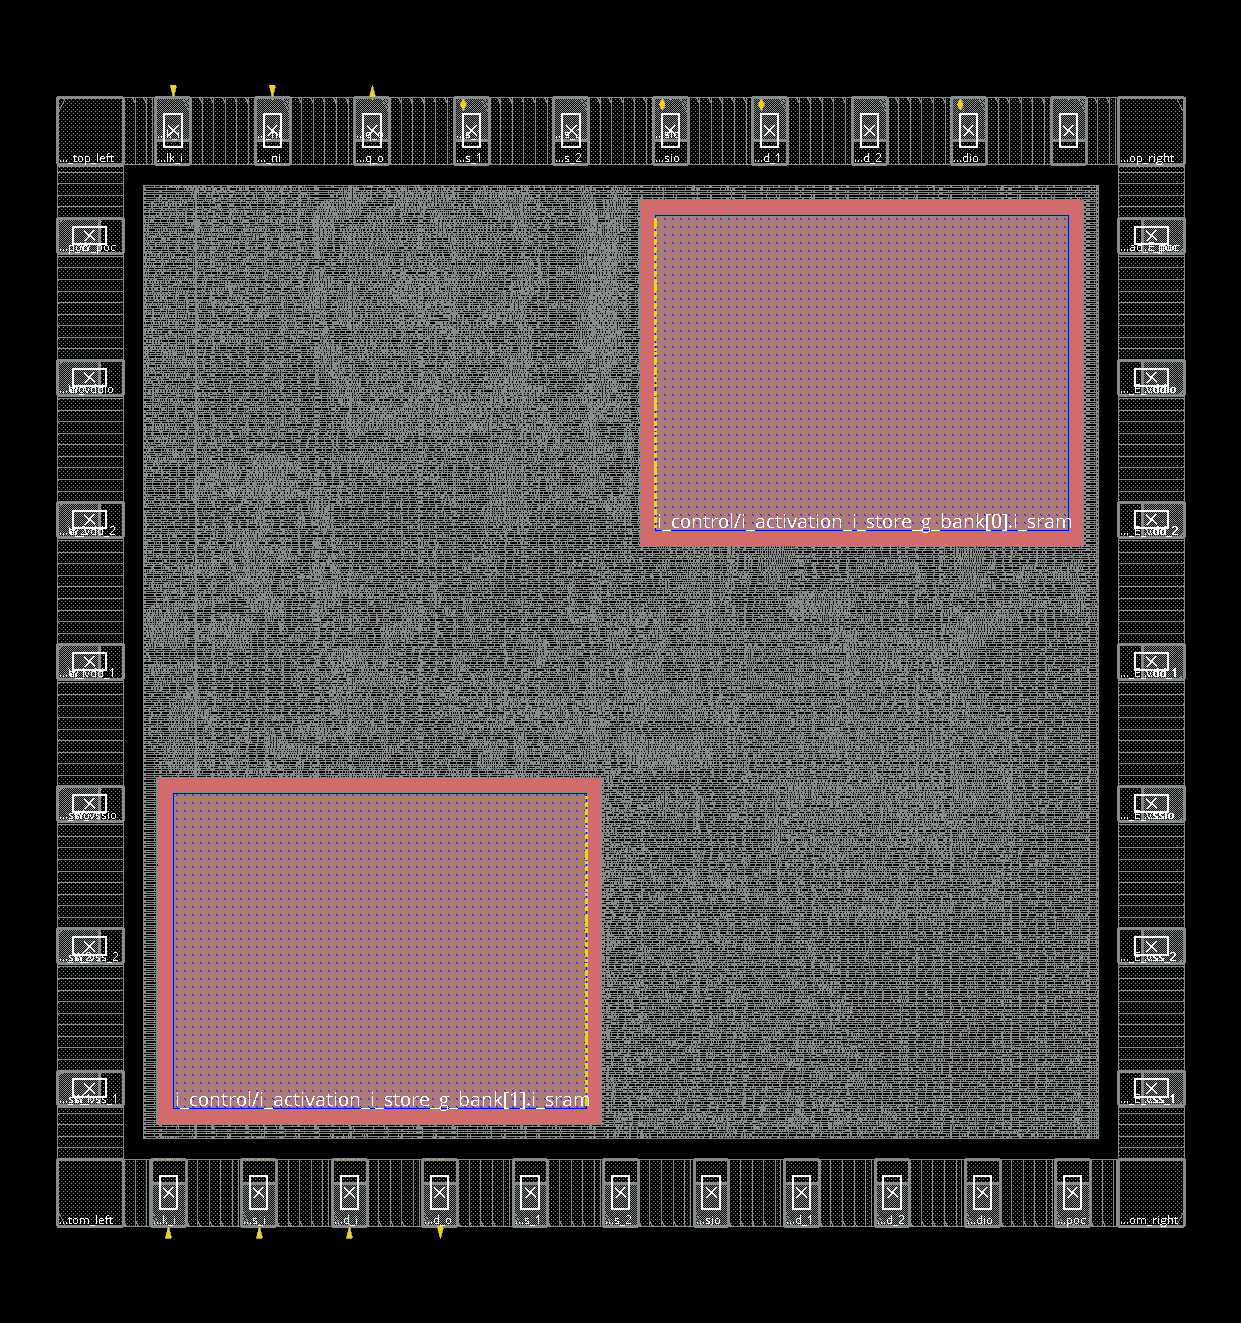
\includegraphics[width=\linewidth]{figs/1_placement.png}\par{\tiny\color{muted} Placement（\NMacroCount{} SRAM 对角放置）}
    \column{0.27\textwidth}
      \centering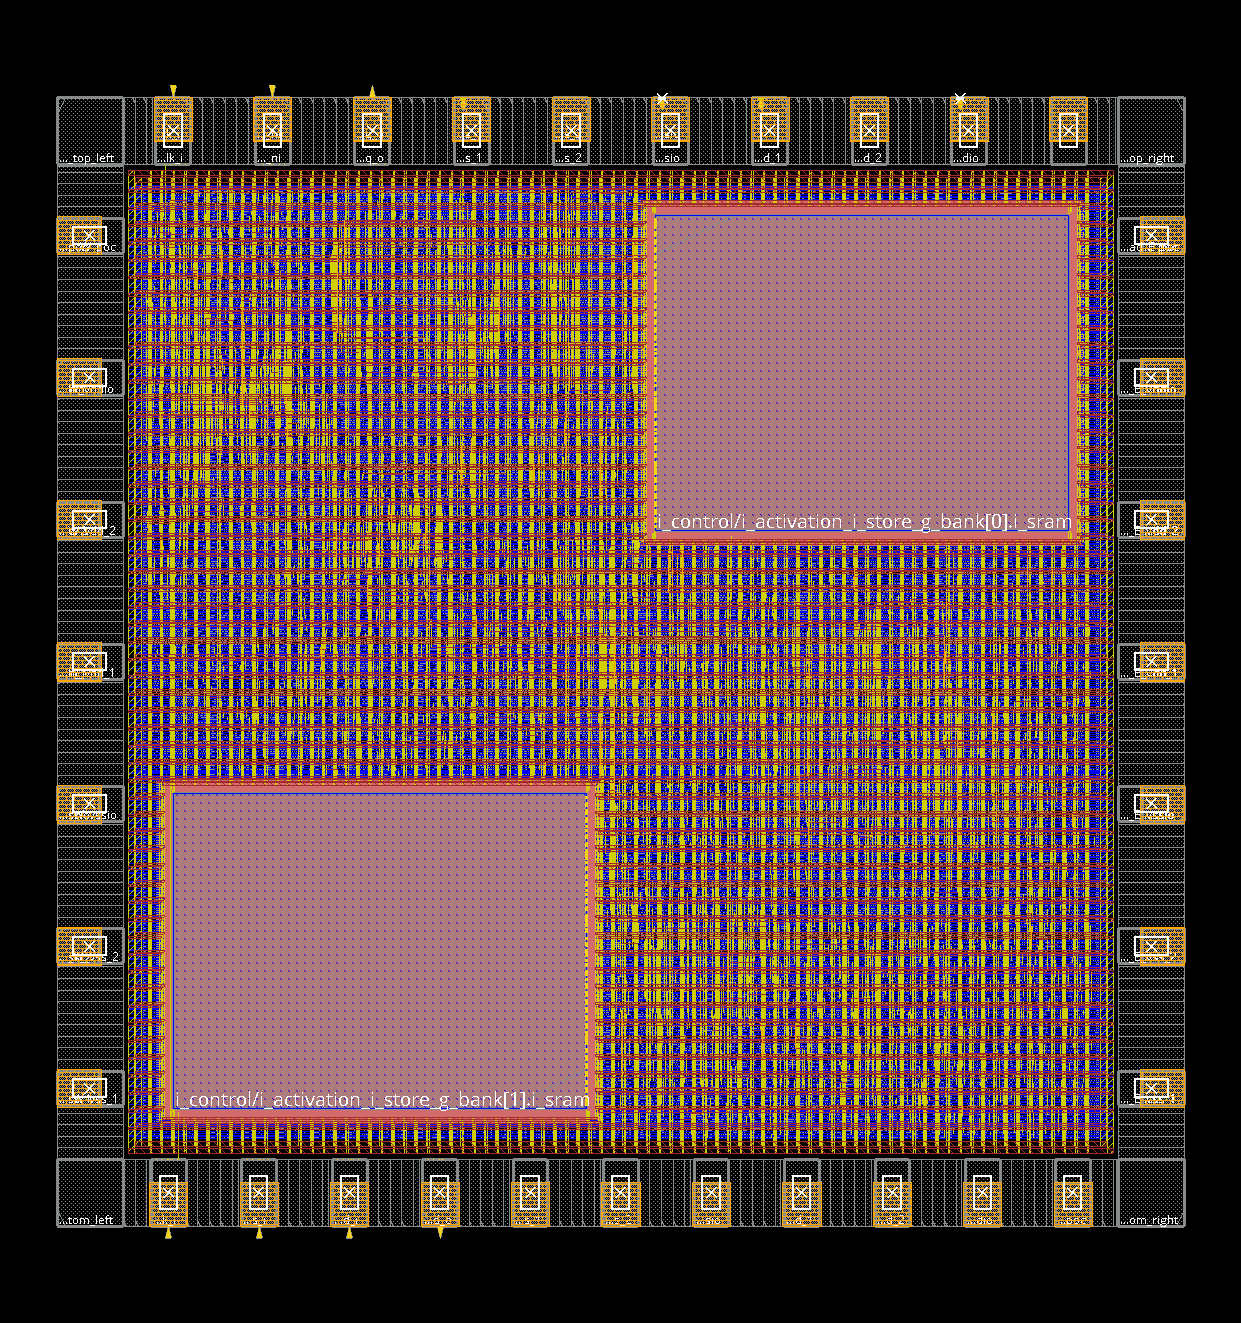
\includegraphics[width=\linewidth]{figs/2_power.png}\par{\tiny\color{muted} Power grid / rings}
    \column{0.42\textwidth}
    {\tiny\setlength{\tabcolsep}{3pt}
    \begin{tabularx}{\linewidth}{@{}>{\raggedright\arraybackslash}X r@{}}
      \toprule
      \textbf{几何 / 面积} & \textbf{值} \\ \midrule
      Active die bbox & \NActiveW{} × \NActiveH{} µm \\
      Sealed die（\tsub{postDummy.gds}） & \hl{\NSealW{} × \NSealH{} µm} \\
      Die / Core area & \NDieMm{} / \NCoreMm{} mm² \\
      Std cells（post-route） & \NStdCells{}，\NStdArea{} mm² \\
      SRAM macros & \NMacroCount{}× \tsub{\NSramMacro}，\NMacroArea{} mm² \\
      Core 占用率（cell+macro） & \NCoreUtil\% \\
      Synth → post-route std 面积 & \NSynthStd{} → \NStdArea{} mm²（+\NCtsRepairPct\%） \\ \bottomrule
    \end{tabularx}}\par\vspace{4pt}
    \begin{tikzpicture}
      \begin{axis}[isscclab, xbar stacked, width=\linewidth, height=1.75cm, xmin=0, xmax=2.0,
          ytick=\empty, axis lines*=none, xtick={0,0.5,1,1.5,2}, xlabel={综合面积 (mm²)}, bar width=9pt,
          legend columns=3, legend style={at={(0.5,1.08)}, anchor=south}]
        \addplot[fill=steel!80, draw=none] coordinates {(\NMacroArea,0)};
        \addplot[fill=peking!80, draw=none] coordinates {(\NFlopArea,0)};
        \addplot[fill=cG!60, draw=none] coordinates {(\NCombArea,0)};
        \legend{Macro \NMacroPct\%, Flop \NFlopPct\%, Comb \NCombPct\%}
      \end{axis}
    \end{tikzpicture}\par\vspace{1pt}
    {\tiny\setlength{\tabcolsep}{3pt}\tabinput{data/area_modules.tex}}
  \end{columns}\par\vspace{3pt}
  \snote{psum 累加器 \NPsumFlops{} 个 FF，占触发器面积 \NPsumFlopPct\%；CTS 与时序修复新增 \NCtsRepair{} k\textmu m² 标准单元面积。}
\end{frame}

% ===================================================================== 09 MMMC
\begin{frame}{4-Corner MMMC 时序闭合与 ±\NRcPct\% RC 敏感度 · Timing Closure}
  \begin{columns}[T,onlytextwidth]
    \column{0.50\textwidth}
    {\small\textbf{Post-route Setup / Hold WNS（\NMmmcViews{} views）}}\par\vspace{2pt}
    \begin{tikzpicture}
      \begin{axis}[isscclab, ybar, width=\linewidth, height=3.7cm, ymin=0, ymax=18, ytick={0,5,10,15},
          xtick={0,1,2,3}, xticklabels={\tsub{ss125}, \tsub{tt25}, \tsub{ff0}, \tsub{ffm40}}, bar width=10pt,
          enlarge x limits=0.18, ylabel={WNS (ns)}, ymajorgrids,
          legend columns=2, legend style={at={(0.5,1.02)}, anchor=south},
          nodes near coords, nodes near coords style={font=\tiny, rotate=90, anchor=west, /pgf/number format/fixed, /pgf/number format/zerofill, /pgf/number format/precision=3}]
        \addplot[fill=peking!85, draw=none] table[x=idx, y=setup] {data/mmmc.dat};
        \addplot[fill=steel!75, draw=none] table[x=idx, y=hold] {data/mmmc.dat};
        \legend{Setup, Hold}
      \end{axis}
    \end{tikzpicture}\par
    \snote{全部 view 违例端点 \NMmmcViol、TNS \NMmmcTns{} ns。最紧 setup 在 \tsub{ss125}（+\NSSSetup{} ns，等效 \NSSFmax{} MHz）；最紧 hold 在 \tsub{ffm40}（+\NFFMHold{} ns）。}
    \column{0.47\textwidth}
    {\small\textbf{RC 缩放敏感度（\tsub{rc\_sensitivity.tsv}）}}\par\vspace{1pt}
    {\tiny\setlength{\tabcolsep}{3.5pt}\renewcommand{\arraystretch}{0.95}\tabinput{data/rc_table.tex}}\par\vspace{2pt}
    \snote{\tsub{ss125} 在 \NRcMax× RC 下 setup 仍为 +\NRcSSWorst{} ns；\tsub{ffm40} 在 \NRcMin× RC 下 hold 仍为 +\NRcFFMWorst{} ns，共 \NRcViol{} 违例。}
    \par\vspace{1pt}
    {\small\textbf{\tsub{\NSramMacro} 接口时序（ns）}}\par\vspace{1pt}
    {\tiny\setlength{\tabcolsep}{2.6pt}\renewcommand{\arraystretch}{0.95}\tabinput{data/sram_table.tex}}\par\vspace{1pt}
    \snote{\NSramPaths{} 组 bank×corner 全部为正，最小 \NSramMinSlack{} ns（Innovus 检查）。}
  \end{columns}
\end{frame}

% ===================================================================== 10 Signoff STA / LEC / SDF
\begin{frame}{等价性、签核 STA 与双角门级 SDF · LEC, STA \& SDF}
  \begin{columns}[T,onlytextwidth]
    \column{0.31\textwidth}
      \card[peking]{PRIMETIME · TT25}{签核 STA}
      \bignum{+\NStaSetup}{ns setup}\par\vspace{1pt}
      \bignum{+\NStaHold}{ns hold}\par\vspace{3pt}
      \begin{itemize}\setlength{\itemsep}{1pt}
        \item 范围：标准单元 + IO；\tsub{unannotated = \NStaUnannot}。
        \item \tsub{\NStaBlackBox} 内部黑盒化，接口由 Innovus MMMC 覆盖。
      \end{itemize}
    \column{0.31\textwidth}
      \card[steel]{FORMALITY}{RTL vs. post-route 网表}
      \bignum{\NLecPass}{LEC verified}\par\vspace{3pt}
      \begin{itemize}\setlength{\itemsep}{1pt}
        \item 证明 CTS、时序修复与填充后网表与 RTL（\tsub{\NAsicCommit}）等价。
        \item 复位修复后的 RTL 即签核 RTL，无额外 ECO。
      \end{itemize}
    \column{0.31\textwidth}
      \card[peking]{XCELIUM · GATE-LEVEL SDF}{双角全芯片 JTAG 回归}
      \bignum{\NSdfPass}{\tsub{ss125\_max} + \tsub{ffm40\_min}}\par\vspace{3pt}
      \begin{itemize}\setlength{\itemsep}{1pt}
        \item 每角 \NSdfJtag{} 条 JTAG 命令（\tsub{\NSdfMtmSs} / \tsub{\NSdfMtmFm} 延迟）。
        \item fatal = \NSdfFatal；无意外 SDFNEP/SDFNET 告警。
        \item 已接受：\NSdfIfnone{} 条 \tsub{ifnone} 路径、\NSdfNegedge{} 条 SRAM negedge period、\NSdfTimeZero{} 个 time-0 输入 pad 冲突。
      \end{itemize}
  \end{columns}\par\vspace{6pt}
  \begin{tikzpicture}[node distance=0.32cm, font=\tiny]
    \node[issccbox=2.25cm, minimum height=0.8cm] (a) {四态 SDF 仿真\\\tsub{ss125\_max}：读回 \texttt{X}};
    \node[issccbox=2.25cm, minimum height=0.8cm, right=of a] (b) {回溯 \texttt{X} 源头\\\tsub{cache\_tag[6]} 被污染};
    \node[issccbox=2.25cm, minimum height=0.8cm, right=of b] (c) {写合并队列 / \tsub{ret2}\\控制寄存器未复位};
    \node[issccbox=2.25cm, minimum height=0.8cm, right=of c, draw=peking, line width=1pt] (d) {PR \#30 复位修复\\仅改复位赋值};
    \node[issccbox=2.25cm, minimum height=0.8cm, right=of d, draw=passink, line width=1pt] (e) {双角 \NSdfJtag-JTAG\\\NSdfPass{} + LEC \NLecPass};
    \foreach \x/\y in {a/b,b/c,c/d,d/e} \draw[issccarr] (\x) -- (\y);
  \end{tikzpicture}
  \par\vspace{3pt}\snote{边界：两角均以 \tsub{timing\_diagnostics = \NSdfTimingDiag} 运行（不启用时序检查停机），各有 \NSdfSramUnq{} 条未限定的 SRAM CLK→Q IOPATH；\tsub{ffm40\_min} 有 \NSdfClampFm{} 条负延迟 IOPATH 被钳位为 0（\tsub{ss125\_max} 为 \NSdfClampSs）。详见第 18 页。}
\end{frame}

% ===================================================================== 11 Calibre
\begin{frame}{Calibre 物理验证与 DFM 收尾 · Physical Verification \& DFM Closure}
  \begin{columns}[T,onlytextwidth]
    \column{0.32\textwidth}
      \centering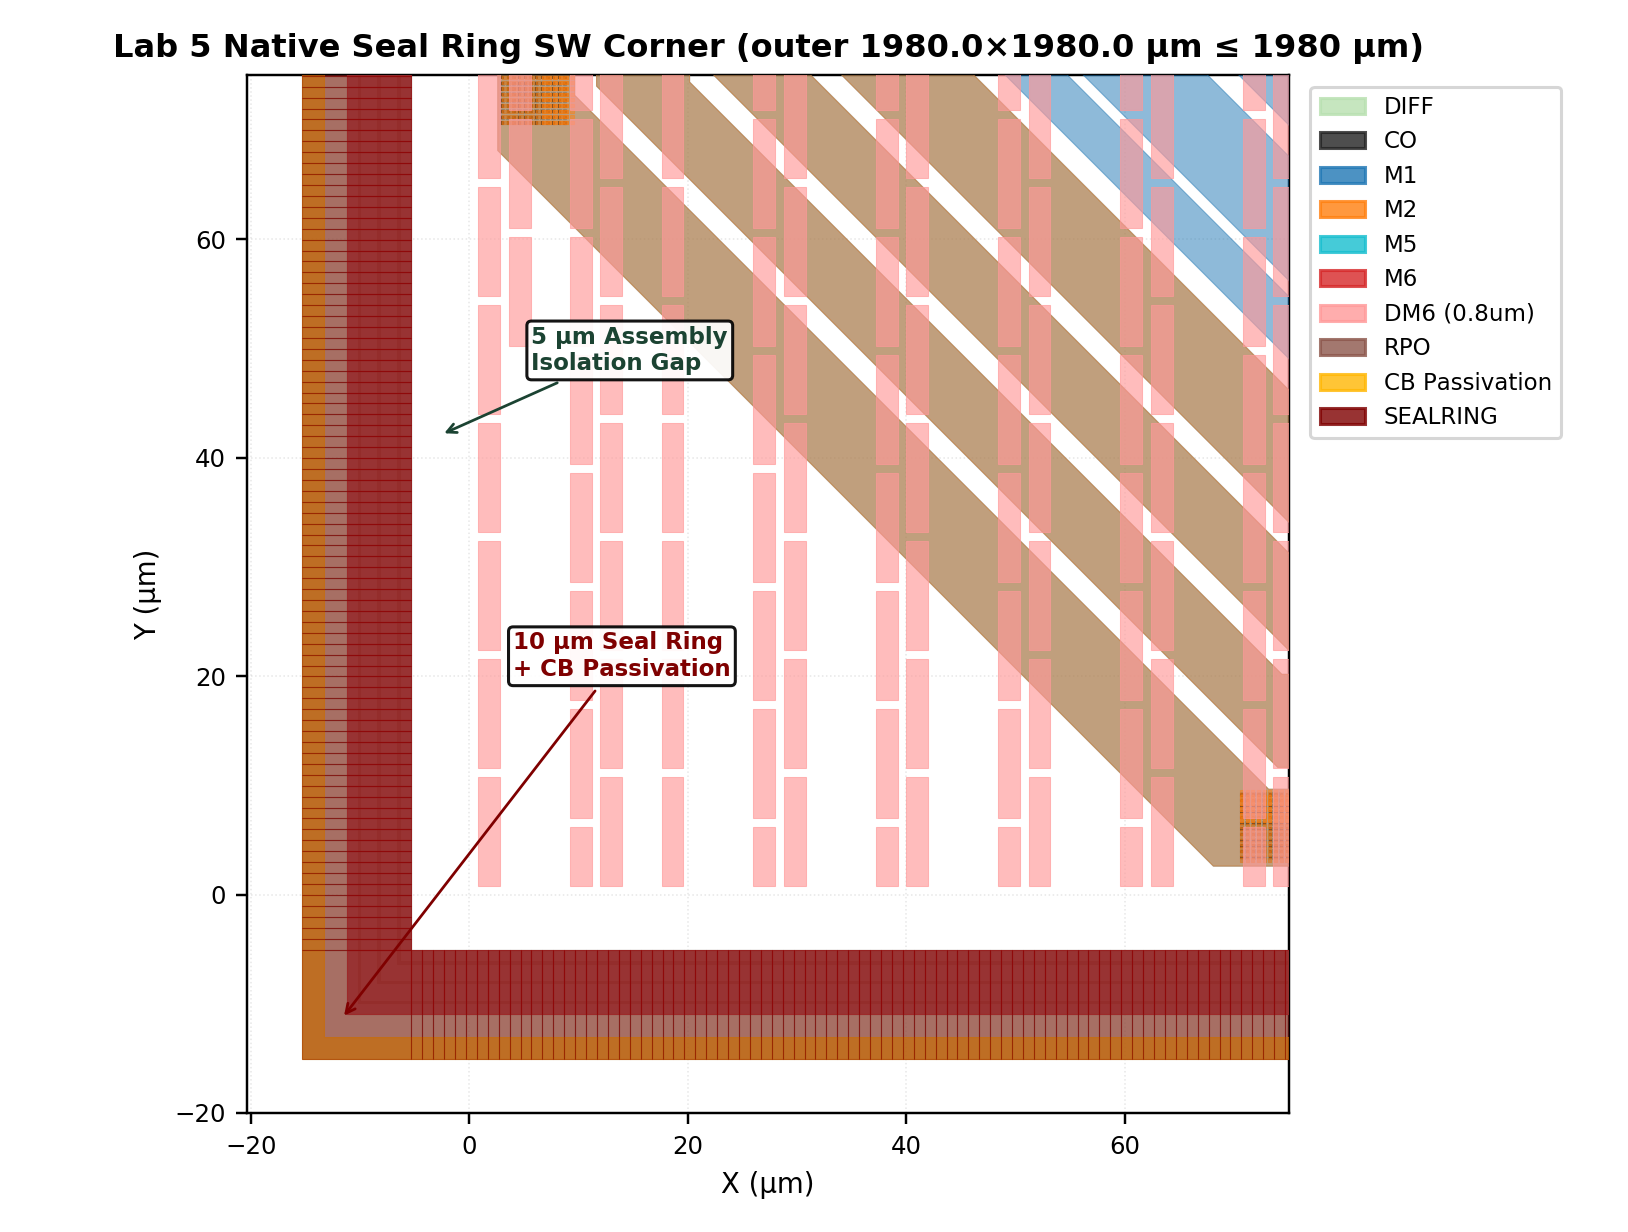
\includegraphics[height=3.45cm]{figs/8_lab5_sealring_corner.png}\par
      {\tiny\color{muted} Seal ring 角部 · sealed \NSealW{}×\NSealH{} µm}
    \column{0.32\textwidth}
      \centering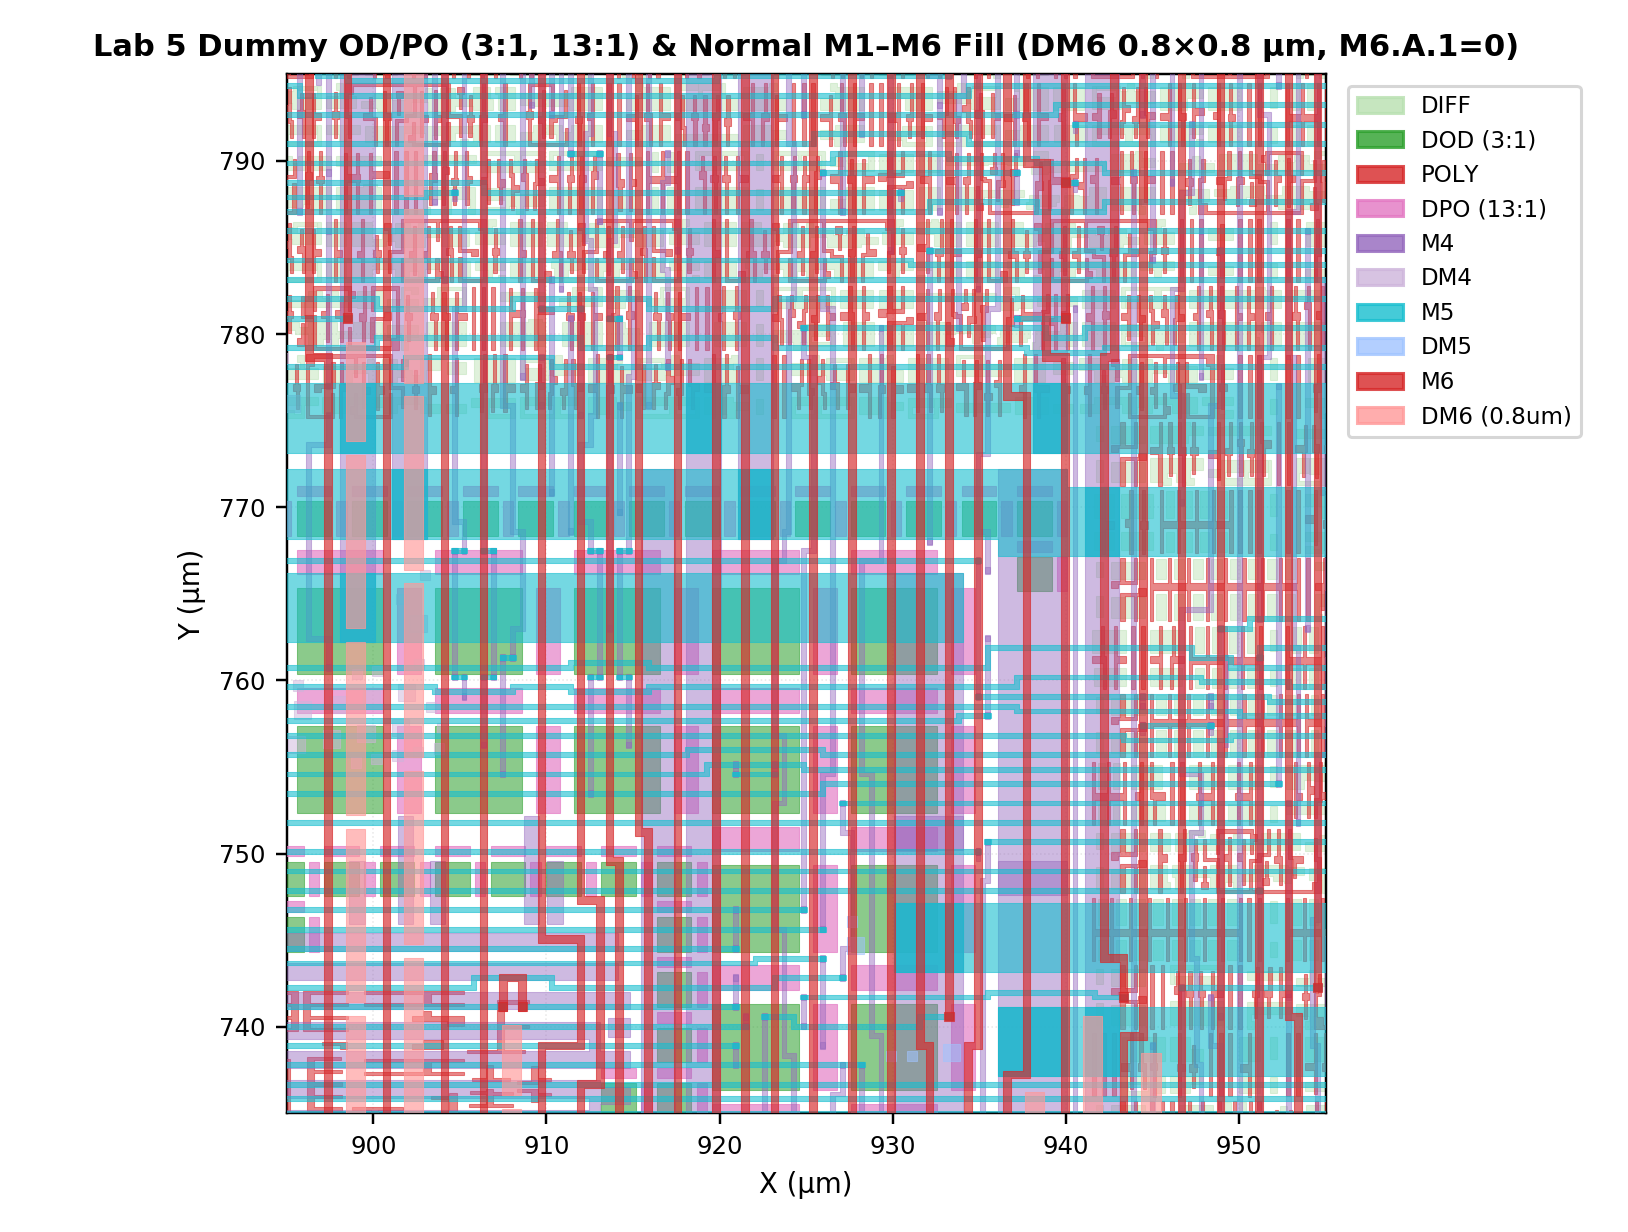
\includegraphics[height=3.45cm]{figs/9_lab5_dummy_fill_zoom.png}\par
      {\tiny\color{muted} Dummy fill · \NFillLayers{} 层（\NFillLayerList）}
    \column{0.32\textwidth}
      \centering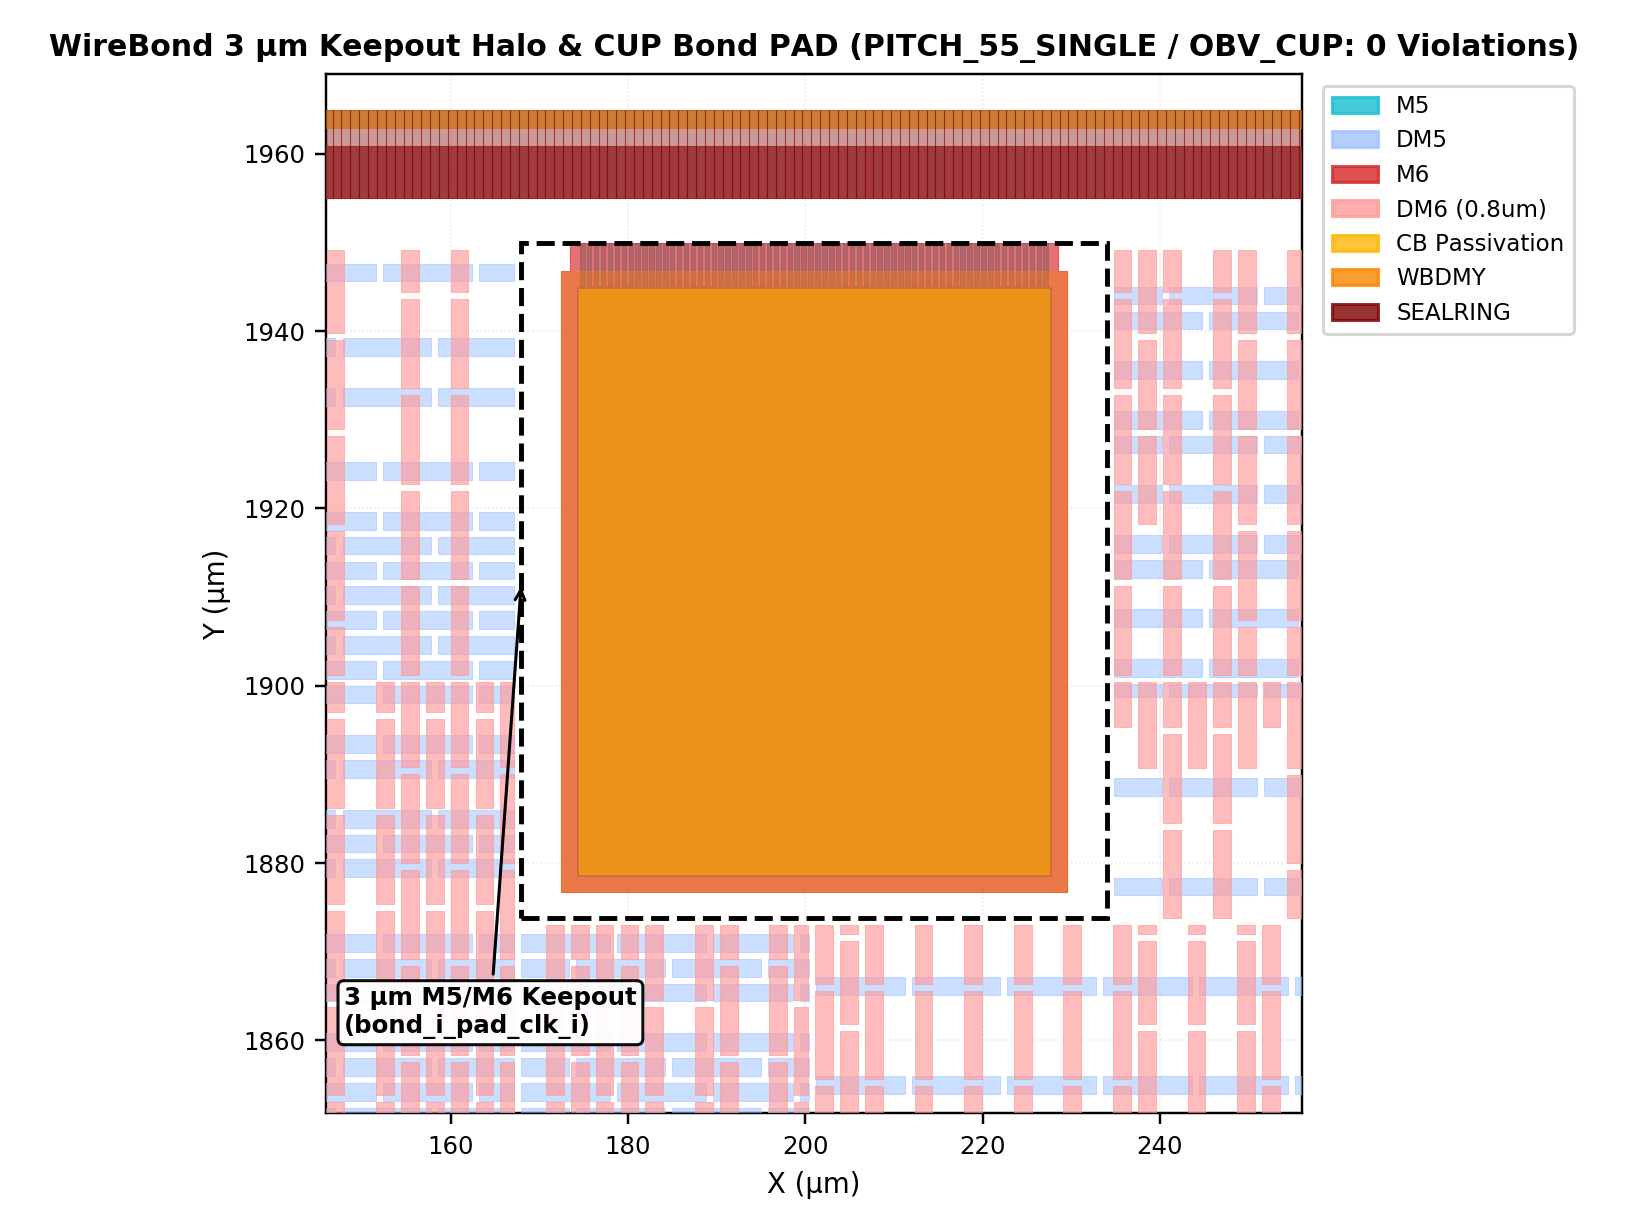
\includegraphics[height=3.45cm]{figs/10_lab5_wirebond_keepout_zoom.png}\par
      {\tiny\color{muted} Wirebond keepout 放大}
  \end{columns}\par\vspace{5pt}
  \begin{columns}[T,onlytextwidth]
    \column{0.235\textwidth}
      \card[peking]{DRC · \NDrcRules{} RULES}{阻断违例}
      \bignum{\NDrcBlocking}{blocking}\par
      {\tiny\color{muted}\NDrcTeachCats{} 类教学 IO/ESD/LUP 类别单列}
    \column{0.235\textwidth}
      \card[steel]{ANTENNA · \NAntRules{} RULES}{天线效应}
      \bignum{\NAntViol}{violations}\par
      {\tiny\color{muted}同源 \tsub{postDummy.gds}}
    \column{0.235\textwidth}
      \card[peking]{WIREBOND · \NWbRules{} RULES}{键合规则}
      \bignum{\NWbViol}{violations}\par
      {\tiny\color{muted}\NDbu{} DBU/µm}
    \column{0.235\textwidth}
      \card[steel]{nmLVS · \NLvsPorts/\NLvsPorts{} PORTS}{SRAM 非黑盒}
      \bignum{\NLvsStatus}{@ \NLvsTol\%}\par
      {\tiny\color{muted}0\% 容差：\NLvsZeroErr{} 个 IO 电阻属性差（≤\NLvsMaxDev\%）}
  \end{columns}\par\vspace{4pt}
  \snote{\tsub{CO.R.4} 修复：IO 单元 \tsub{\NCorCell} 的接触孔未被 PIMP 覆盖，补 PP 矩形 [\NCorPatch] µm，右边界贴齐相邻 NP 墙 \NCorNpWall{} µm。}
\end{frame}

% ===================================================================== 12 Power
\begin{frame}{100\%-VCD 五负载布线后功耗与融合节能 · Post-Layout Power}
  \begin{columns}[T,onlytextwidth]
    \column{0.49\textwidth}
    {\small\textbf{功耗拆分（mW，TT25，\NAsicClk{} MHz）}}\par\vspace{1pt}
    \begin{tikzpicture}
      \begin{axis}[isscclab, ybar stacked, width=\linewidth, height=4.2cm, ymin=0, ymax=52,
          xtick=data, xticklabels from table={data/power.dat}{name}, bar width=13pt, enlarge x limits=0.14,
          ylabel={Power (mW)}, ymajorgrids, legend columns=2, legend style={at={(0.5,1.02)}, anchor=south}]
        \addplot[fill=peking!85, draw=none] table[x=idx, y=internal] {data/power.dat};
        \addplot[fill=steel!75, draw=none] table[x=idx, y=switching] {data/power.dat};
        \legend{Internal, Switching}
      \end{axis}
    \end{tikzpicture}\par
    \snote{总功耗 \NPowMin–\NPowMax{} mW；漏电约 \NLeakUw{} µW。Vectorless 估计为 \NVecPower{} mW，偏保守。}
    \column{0.49\textwidth}
    {\small\textbf{单次推理能量（µJ，对数轴）}}\par\vspace{1pt}
    \begin{tikzpicture}
      \begin{axis}[isscclab, ybar, width=\linewidth, height=4.2cm, ymode=log, ymin=0.1, ymax=100,
          log origin=infty, xtick=data, xticklabels from table={data/power.dat}{name}, bar width=13pt, enlarge x limits=0.14,
          ylabel={Energy (µJ)}, ymajorgrids,
          nodes near coords, nodes near coords style={font=\tiny, /pgf/number format/fixed, /pgf/number format/zerofill, /pgf/number format/precision=2},
          point meta=explicit]
        \addplot[fill=steel!75, draw=none] table[x=idx, y=energy, meta=energy] {data/power.dat};
      \end{axis}
    \end{tikzpicture}\par
    \snote{能量 = 平均功耗 × \tsub{busy→irq} 窗口；\NVcdCount{} 个负载 VCD 注释率均为 \NVcdAct\%。}
  \end{columns}\par\vspace{2pt}
  \callout[passink]{\textbf{算子融合节能 \hl{\NFuseSave\%}}：同一 CNN 融合版 \tsub{cnn\_f1} 周期 \NFZeroCyc{} → \NFOneCyc{}（−\NFuseCycPct\%）。平均功耗由 \NFZeroP{} 升到 \NFOneP{} mW（阵列更忙），但单次能量 \NFZeroE{} → \hl{\NFOneE{} µJ}。}
\end{frame}

% ===================================================================== 13 FPGA TCK sweep
\begin{frame}{\NSysClk{} MHz EGo1 实板与 MPSSE TCK 扩展 · Live FPGA TCK Sweep}
  \begin{columns}[T,onlytextwidth]
    \column{0.315\textwidth}
    {\small\textbf{冷加载 load\_model（ms）}}\par
    \begin{tikzpicture}
      \begin{axis}[isscclab, width=1.08\linewidth, height=4.1cm, xmode=log, log basis x=10,
          xtick={1,2,3,5,8,10,15}, xticklabels={1,2,3,5,8,10,15}, xlabel={TCK (MHz)}, ymin=30, ymax=160,
          ymajorgrids, cycle list={{cA,mark=*},{cB,mark=square*},{cC,mark=triangle*},{cD,mark=diamond*},{cE,mark=pentagon*},{cF,mark=o},{cG,mark=x}},
          every axis plot/.append style={line width=0.7pt, mark size=1.2pt}]
        \foreach \c in {ecg,har,mnistl,fashioncnn,kwsm,kwsl,gtsrbl} {\addplot table[x=tck, y=\c] {data/tck_load.dat};}
      \end{axis}
    \end{tikzpicture}
    \column{0.315\textwidth}
    {\small\textbf{热推理 warm median（ms）}}\par
    \begin{tikzpicture}
      \begin{axis}[isscclab, width=1.08\linewidth, height=4.1cm, xmode=log, log basis x=10,
          xtick={1,2,3,5,8,10,15}, xticklabels={1,2,3,5,8,10,15}, xlabel={TCK (MHz)}, ymin=10, ymax=46,
          ymajorgrids, cycle list={{cA,mark=*},{cB,mark=square*},{cC,mark=triangle*},{cD,mark=diamond*},{cE,mark=pentagon*},{cF,mark=o},{cG,mark=x}},
          every axis plot/.append style={line width=0.7pt, mark size=1.2pt},
          legend columns=1, legend style={at={(1.02,1)}, anchor=north west, font=\tiny}, legend cell align=left]
        \foreach \c in {ecg,har,mnistl,fashioncnn,kwsm,kwsl,gtsrbl} {\addplot table[x=tck, y=\c] {data/tck_warm.dat};}
      \end{axis}
    \end{tikzpicture}
    \column{0.33\textwidth}
    {\small\textbf{FPGA BRAM vs. 行为级 SRAM 周期}}\par\vspace{1pt}
    {\tiny\setlength{\tabcolsep}{2.4pt}\tabinput{data/cycle_delta.tex}}\par\vspace{1pt}
    \snote{同步 BRAM 每次张量读多 1 拍，周期 +\NCycDeltaMin–\NCycDeltaMax\%；输出逐位相同（RTL 审计 \NAuditExact/\NAuditFrames{} 帧）。}
  \end{columns}\par\vspace{1pt}
  {\tiny\color{muted}\textcolor{cA}{■}\,\tsub{ecg}\enspace\textcolor{cB}{■}\,\tsub{har}\enspace\textcolor{cC}{■}\,\tsub{mnist\_l}\enspace\textcolor{cD}{■}\,\tsub{fashion\_cnn}\enspace\textcolor{cE}{■}\,\tsub{kws\_m}\enspace\textcolor{cF}{■}\,\tsub{kws\_l}\enspace\textcolor{cG}{■}\,\tsub{gtsrb\_l}}\par\vspace{2pt}
  \callout[peking]{\NZooModels{} 模型 × \NTckCount{} 档 TCK × \NZooFramesPer{} 次（1 冷 + \NZooWarm{} 热）= \hl{\NZooExact/\NZooRuns{} 次 0-bit 精确}。冷加载几何均值 \NLoadGeoLo{} → \NLoadGeoHi{} ms（\NTckMin→\NTckMax{} MHz，\NLoadSpeedup×）；热推理仅 \NWarmGeoLo{} → \NWarmGeoHi{} ms，说明单帧延迟已被 USB 往返与轮询而非 TCK 主导。}
\end{frame}

% ===================================================================== 14 Scenes
\begin{frame}{实板边缘应用：六场景演示 · Live Edge Applications on EGo1}
  \begin{columns}[T,onlytextwidth]
    \column{0.64\textwidth}
    {\small\textbf{六场景代表帧实板结果（TCK \NSceneTck{} MHz）}}\par\vspace{2pt}
    {\tiny\setlength{\tabcolsep}{3pt}\tabinput{data/scenes.tex}}\par\vspace{3pt}
    \snote{NPU ms = 中位周期 ÷ \NSysClk{} MHz；Med./p95 为端到端单帧延迟；Xfer 为 JTAG 传输中位数；fps 为平均吞吐。}
    \column{0.33\textwidth}
      \card[peking]{GOLDEN AGREEMENT}{逐位一致}
      \bignum{\NSceneExact/\NSceneFrames}{frames}\par
      {\scriptsize\color{muted}\tsub{agreement\_rate = \NSceneAgree}}\par\vspace{5pt}
      \card[steel]{LATENCY / THROUGHPUT}{端到端}
      \bignum{\NSceneMedMin–\NSceneMedMax}{ms 中位}\par
      \bignum{\NSceneFpsMin–\NSceneFpsMax}{fps 平均}\par
  \end{columns}\par\vspace{5pt}
  \callout[warnink]{\textbf{范围说明（\tsub{scope\_note}）}：\NSceneScope。这些是六个演示场景公开的 golden 输入，检查的是 NPU 输出与 golden 输出逐位相等，\textbf{不是}数据集分类准确率。离线全量检查另有 \NZooGolden{} zoo golden 帧。单帧 NPU 计算 ≤ \NSceneNpuMax{} ms，其余时间是 USB/JTAG 传输与轮询。}
\end{frame}

% ===================================================================== 15 ResNet-20
\begin{frame}{实板深度残差推理：ResNet-20 · Live Deep Residual Inference on EGo1}
  \begin{columns}[T,onlytextwidth]
    \column{0.52\textwidth}
    {\small\textbf{CIFAR-10 INT4 QAT · \NRTwSamples{} 帧实板结果（TCK \NRTwTck{} MHz）}}\par\vspace{2pt}
    {\tiny\setlength{\tabcolsep}{3pt}\tabinput{data/resnet20_rows.tex}}\par\vspace{3pt}
    \snote{\NRTwSamples/\NRTwSamples{} 帧 \tsub{bit\_exact = \NRTwExact}、\tsub{max\_abs\_diff = \NRTwMaxDiff}；标签正确 \NRTwLabel/\NRTwSamples（第 \NRTwMissIdx{} 号帧是模型本身误判，硬件输出仍与参考逐位一致）。}
    \par\vspace{3pt}
    {\scriptsize
    \begin{tabular}{@{}lr@{}}
      \toprule
      \textbf{每帧计划} & \textbf{值} \\ \midrule
      Program groups / Tile calls & \NRTwHwGroups{} / \NRTwHwTiles \\
      Fused subgraphs / Host ops & \NRTwHwFused{} / \NRTwHwHostOps \\
      JTAG bytes（实测 = 计划） & \NRTwMeasBytes \\ \bottomrule
    \end{tabular}}
    \column{0.45\textwidth}
    {\small\textbf{中位单帧时间拆分（ms，对数轴）}}\par\vspace{2pt}
    \begin{tikzpicture}
      \begin{axis}[isscclab, xbar, width=\linewidth, height=3.1cm, xmode=log, xmin=1, xmax=200000, log origin=infty, nodes near coords align=horizontal,
          ytick={0,1,2}, yticklabels={Host, NPU compute, USB/JTAG}, bar width=9pt, enlarge y limits=0.3,
          xlabel={ms}, xmajorgrids, nodes near coords, point meta=explicit,
          nodes near coords style={font=\tiny, /pgf/number format/fixed, /pgf/number format/precision=2, /pgf/number format/1000 sep={,}}]
        \addplot[fill=steel!80, draw=none] table[x=ms, y=idx, meta=ms] {data/resnet20_bd.dat};
      \end{axis}
    \end{tikzpicture}\par\vspace{3pt}
    \callout[peking]{\NRTwCycles{} 周期 = \hl{\NRTwCompute{} ms} NPU 计算（@\NSysClk{} MHz），而墙钟中位 \NRTwWall{} ms，其中 \hl{\NRTwJtagPct\%} 为 USB/JTAG 传输与完成轮询；实测有效带宽约 \NRTwBw{} kB/s。}
  \end{columns}
\end{frame}

% ===================================================================== 16 ResNet-18
\begin{frame}{ImageNet 级 ResNet-18 @ \NSramKB{} KB 片上 SRAM · Scaling to ResNet-18}
  \begin{columns}[T,onlytextwidth]
    \column{0.50\textwidth}
    {\small\textbf{Imagenette INT4 QAT · 实板代表帧}}\par\vspace{2pt}
    {\tiny\setlength{\tabcolsep}{3pt}\renewcommand{\arraystretch}{1.05}
    \begin{tabularx}{\linewidth}{@{}>{\raggedright\arraybackslash}X r@{}}
      \toprule
      \textbf{指标} & \textbf{值} \\ \midrule
      \tsub{samples\_checked} & \hl{\NREiSamples} \\
      \tsub{bit\_exact} / \tsub{max\_abs\_diff} & \NREiExact{} / \NREiMaxDiff \\
      label / predicted & \NREiLabelTrue{} / \NREiPred \\
      NPU cycles & \NREiCycles \\
      NPU compute @\NSysClk{} MHz & \NREiCompute{} ms \\
      Wall / JTAG / Host & \NREiWallS{} s / \NREiJtagS{} s / \NREiHost{} ms \\ \midrule
      Groups 计划 → model loads 实测 & \NREiPlanGroups{} → \NREiLoads \\
      Tile infers & \NREiTileInf \\
      JTAG bytes 计划 / 实测 & \NREiPlanBytes{} / \NREiMeasBytes \\
      \quad model / in / out（实测） & \NREiModelMeas{} / \NREiInBytes{} / \NREiOutBytes \\ \bottomrule
    \end{tabularx}}\par\vspace{2pt}
    \snote{实测比计划少 \NREiModelSaved{} B：运行时检测到相同模型已驻留，\NREiPlanGroups{} 个 group 中只需 \NREiLoads{} 次加载。}
    \column{0.47\textwidth}
    {\small\textbf{计算 vs. 传输（Roofline 式诊断）}}\par\vspace{2pt}
    \begin{tikzpicture}
      \begin{axis}[isscclab, xbar, width=\linewidth, height=3.0cm, xmode=log, xmin=0.1, xmax=20000, log origin=infty, nodes near coords align=horizontal,
          ytick={0,1,2}, yticklabels={Host, NPU compute, USB/JTAG}, bar width=9pt, enlarge y limits=0.3,
          xlabel={s}, xmajorgrids, nodes near coords, point meta=explicit,
          nodes near coords style={font=\tiny, /pgf/number format/fixed, /pgf/number format/precision=2}]
        \addplot[fill=peking!80, draw=none] table[x=s, y=idx, meta=s] {data/resnet18_bd.dat};
      \end{axis}
    \end{tikzpicture}\par\vspace{2pt}
    \begin{itemize}\setlength{\itemsep}{1pt}
      \item 传输占墙钟 \hl{\NREiJtagPct\%}，是计算时间的 \NREiRatio×。
      \item 实测有效带宽 \NREiBw{} kB/s；若要让 \NREiMeasMB{} MB/帧 的数据完全藏在 \NREiComputeShort{} ms 计算之下，需要约 \NREiNeedBw{} MB/s。
      \item 结论：该系统处于传输受限区，下一步应改数据通路而非算力。
    \end{itemize}
  \end{columns}\par\vspace{1pt}
  \callout[warnink]{\textbf{证据范围}：归档收据仅 \tsub{samples\_checked = \NREiSamples}（单帧 \tsub{passed}、\tsub{fpga\_validated}）。未归档的多帧压力测试在 \tsub{usbipd-win} 长时间批量传输中出现 USB 超时，不计入本页结论。}
\end{frame}

% ===================================================================== 17 Cross-platform
\begin{frame}{跨平台 PPA 与全栈协同优化总结 · Cross-Platform PPA}
  \noindent{\scriptsize\setlength{\tabcolsep}{3pt}\renewcommand{\arraystretch}{1.12}%
  \begin{tabularx}{\textwidth}{@{}>{\raggedright\arraybackslash}p{50pt} >{\raggedright\arraybackslash}p{82pt} >{\raggedright\arraybackslash}X >{\raggedright\arraybackslash}X@{}}
    \toprule
    \textbf{维度} & \textbf{RTL 行为级参考} & \textbf{EGo1 FPGA（实板）} & \textbf{TSMC 180 nm ASIC（签核）} \\ \midrule
    时钟 / 存储 & 组合读 SRAM 模型 & \NSysClk{} MHz，同步 BRAM，DSP48E1 MAC & \NAsicClk{} MHz，\NMacroCount{}× \tsub{RA1SHD} \NSramMacroKB{} KB SRAM \\
    验证 & \NAuditExact/\NAuditFrames{} zoo 帧 0-bit；\NProbeExact/\NProbeCount{} ResNet-18 子图 & \NZooExact/\NZooRuns{} zoo 推理、\NSceneExact/\NSceneFrames{} 场景帧、R20 \NRTwSamples/\NRTwSamples、R18 \NREiSamples{} 帧 & LEC \NLecPass；双角 SDF \NSdfJtag-JTAG \NSdfPass \\
    \tsub{ecg} 周期 / 计算 & \NEcgRtlCyc{} 周期 & \NEcgFpgaCyc{} 周期 = \NEcgFpgaUs{} µs（端到端 \NEcgSceneMs{} ms） & \NEcgRtlCyc{} 周期 = \NAsicEcgUs{} µs，\NAsicEcgP{} mW，\NAsicEcgE{} µJ \\
    \tsub{mnist\_l} 计算 / 能量 & \NMnistRtlCyc{} 周期 & 见第 13 页（+\NCycDeltaMin–\NCycDeltaMax\% 周期） & \NAsicMnistUs{} µs，\NAsicMnistP{} mW，\NAsicMnistE{} µJ \\
    ResNet-20 单帧 & \NRTwRtlCyc{} 周期（\tsub{\NProbeCommit}，exact = \NRTwRtlExact） & \NRTwCycles{} 周期 = \NRTwFpgaMs{} ms；墙钟 \NRTwWall{} ms & 按同周期折算 \NRTwAsicMs{} ms（未测功耗） \\
    ResNet-18 单帧 & 子图探针级 & \NREiCycles{} 周期 = \NREiCompute{} ms；墙钟 \NREiWallS{} s & 按同周期折算 \NREiAsicMs{} ms（未测功耗） \\
    面积 / 时序 & — & XC7A35T 实现通过 & 签核 die \NSealW{}×\NSealH{} µm；\NStdCells{} cells；\NMmmcViol{} MMMC 违例 \\ \bottomrule
  \end{tabularx}}\par\vspace{6pt}
  \callout[peking]{\textbf{同一 RTL、三个平台、逐位一致}：FPGA 比行为级多 \NCycDeltaMin–\NCycDeltaMax\% 周期（BRAM 同步读），ASIC 与行为级周期一致。ResNet 的 ASIC 时间按周期 ÷ \NAsicClk{} MHz 折算，未做门级功耗仿真，表中如实标注。}
\end{frame}

% ===================================================================== 18 Boundaries & roadmap
\begin{frame}{工程签核边界与后续演进 · {\normalsize Engineering Signoff Boundaries \& Roadmap}}
  \begin{columns}[T,onlytextwidth]
    \column{0.55\textwidth}
    {\small\textbf{\color{warnink}开放边界审计（\tsub{formal\_tapeout\_signoff = \NFormalTapeout}）}}\par\vspace{2pt}
    {\tiny\setlength{\tabcolsep}{3pt}\renewcommand{\arraystretch}{1.08}
    \begin{tabularx}{\linewidth}{@{}l >{\raggedright\arraybackslash}X@{}}
      \toprule
      \textbf{ERC} & \NErcHier{} hier / \NErcExp{} expanded 标记（\NErcMarkerRules{} 条规则），全部在 IO/封环周边，状态 \tsub{\NErcStatus} \\
      \textbf{LVS} & 0\% 电阻容差下 \NLvsZeroErr{} 个 IO 电阻属性差（最大 \NLvsMaxDev\%），\NLvsTol\% 容差下 \NLvsStatus \\
      \textbf{DRC} & \NDrcTeachCats{} 类教学 IO/ESD/LUP 类别作为豁免单列，需 foundry waiver \\
      \textbf{SDF} & \tsub{timing\_diagnostics = \NSdfTimingDiag}；每角 \NSdfSramUnq{} 条 SRAM CLK→Q IOPATH 未限定；\tsub{ffm40\_min} 钳位 \NSdfClampFm{} 条负 IOPATH \\
      \textbf{RC / IR} & ±\NRcPct\% 为代理 RC 缩放；独立 xRC SPEF 与 PGV/Voltus 静态+动态 IR/EM 尚未执行 \\
      \textbf{实板} & 场景为代表帧；ResNet-18 仅 \NREiSamples{} 帧收据；数小时 USB/IP 压力稳定性未验证 \\ \bottomrule
    \end{tabularx}}\par\vspace{3pt}
    \centering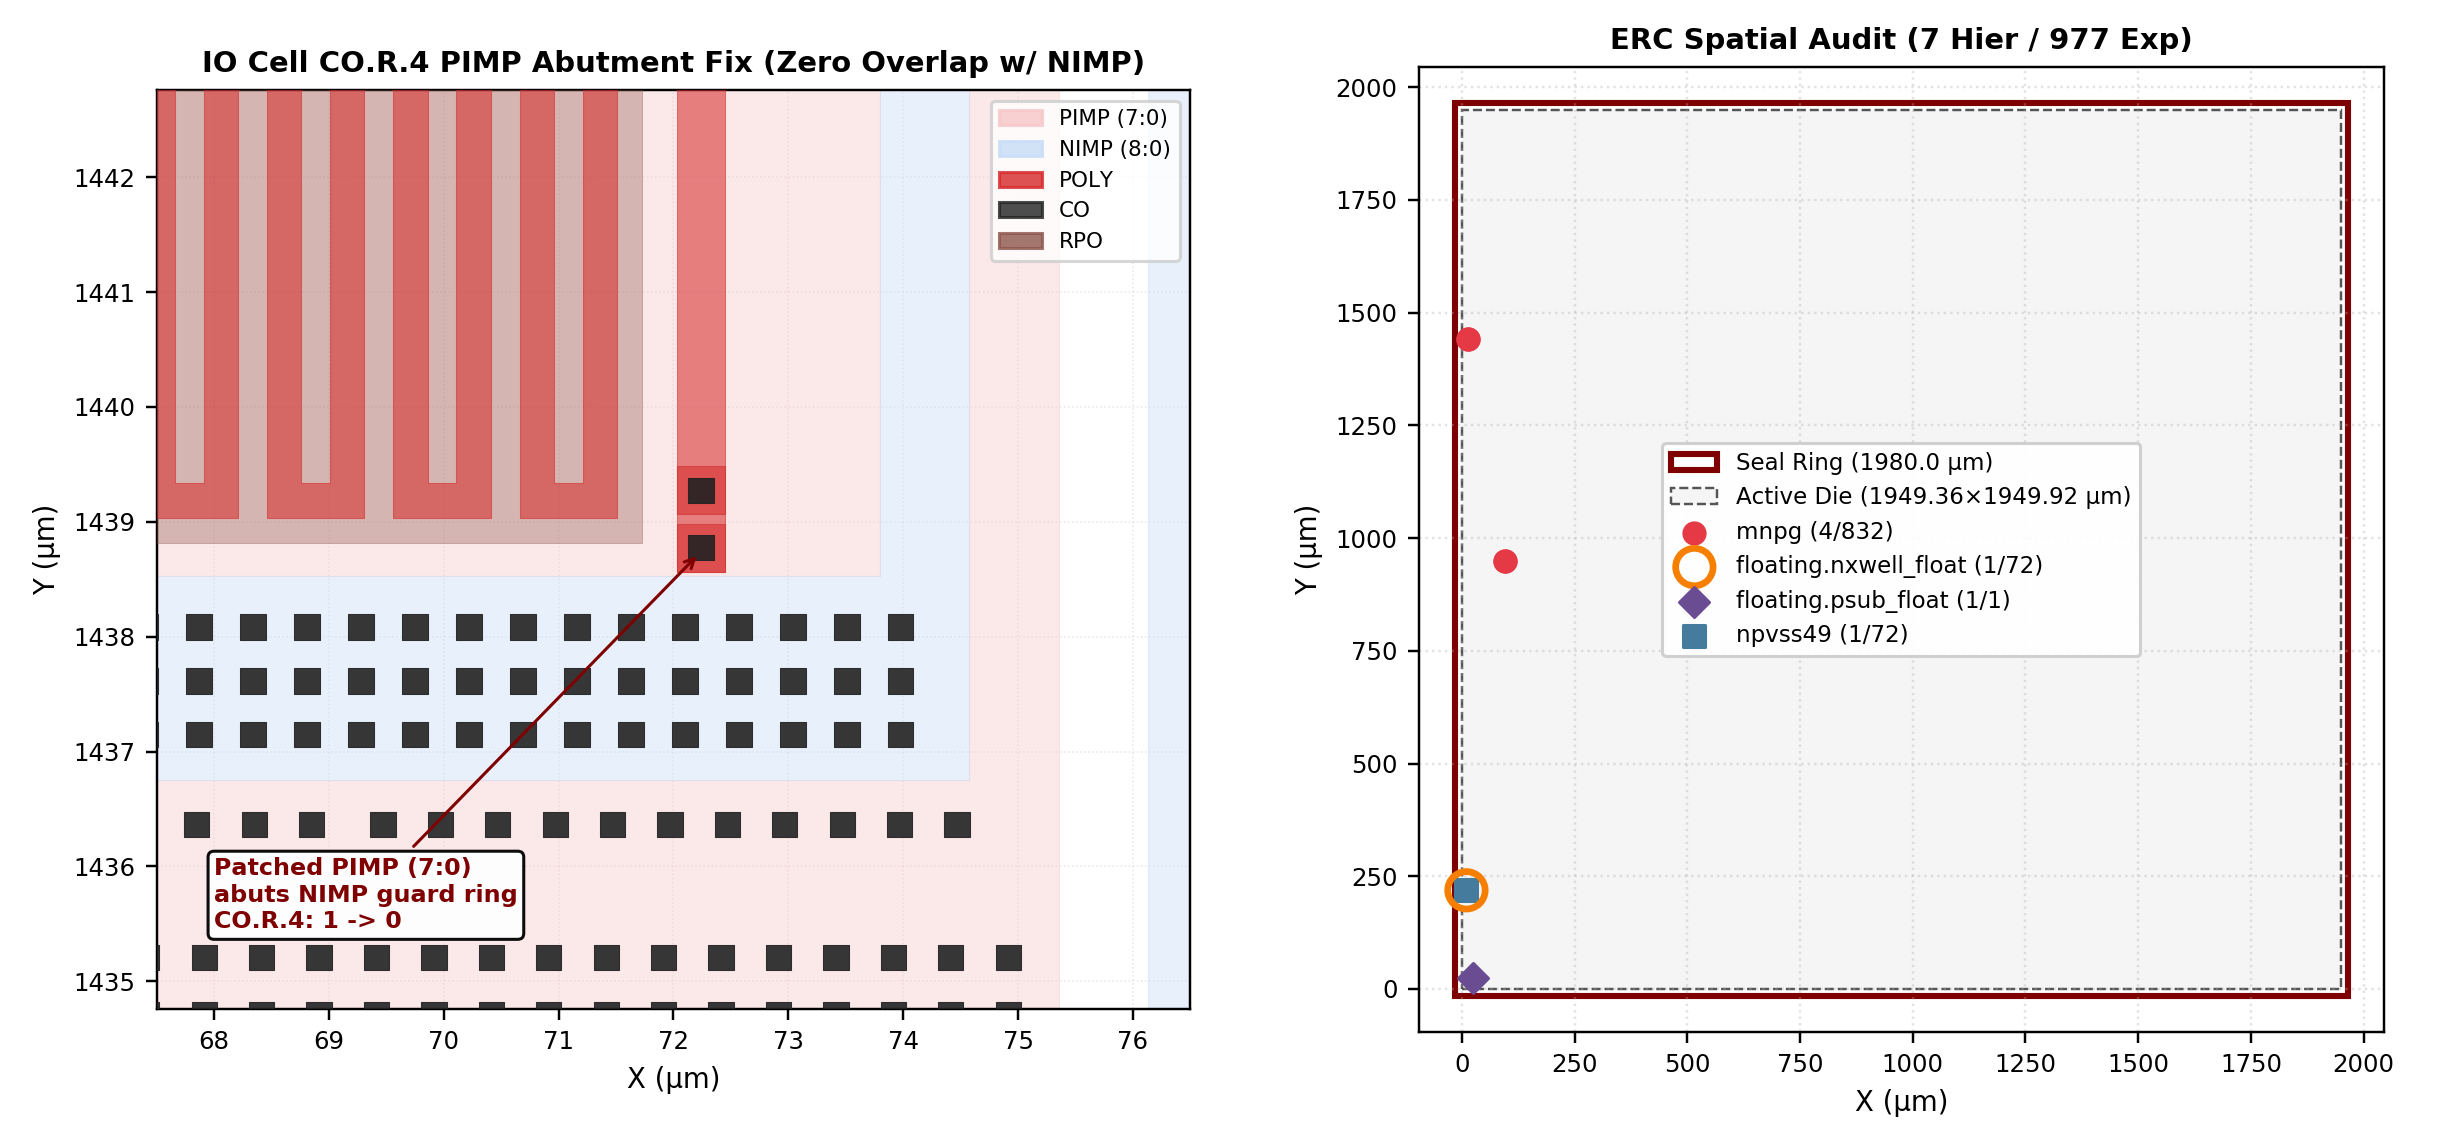
\includegraphics[width=0.70\linewidth]{figs/11_lab5_cor4_and_erc_audit.png}\par
    {\tiny\color{muted}\tsub{CO.R.4} 修复与 ERC 标记位置：均位于 IO/封环，不在核心逻辑与 SRAM 内}
    \column{0.42\textwidth}
    {\small\textbf{\color{peking}架构与签核路线图}}\par\vspace{1pt}
    \card[peking]{01 · DATA PATH}{以 QSPI/DMA 取代 JTAG 数据通路}
    \begin{itemize}\setlength{\itemsep}{1pt}
      \item 权重/激活经片外 QSPI 流式加载、DMA 写入统一 SRAM；JTAG 只做控制与调试。
      \item 释放已测计算能力：ResNet-20 \NRTwComputeShort{} ms、ResNet-18 \NREiComputeShort{} ms；藏住传输需约 \NREiNeedBw–\NRTwNeedBw{} MB/s。
    \end{itemize}\par\vspace{3pt}
    \card[steel]{02 · SIGNOFF}{补齐流片级签核}
    \begin{itemize}\setlength{\itemsep}{1pt}
      \item Calibre xRC SPEF 重跑 MMMC/SDF；Voltus 静态/动态 IR-drop 与 EM。
      \item 打开 SDF 时序检查，限定 SRAM CLK→Q 路径。
      \item LVS 0\% 电阻容差闭合；ERC 与 DRC 教学类别取得 waiver。
      \item 原生 Linux USB 主机上补做 ResNet-18 多帧与长时压力测试。
    \end{itemize}\par\vspace{3pt}
  \end{columns}
\end{frame}

% ===================================================================== 19 Conclusion
\begin{frame}{结论与答辩 · Conclusion \& Q\&A}
  \begin{columns}[T,onlytextwidth]
    \column{0.58\textwidth}
    {\small\textbf{答辩要点}}\par\vspace{2pt}
    \begin{enumerate}\setlength{\itemsep}{3pt}\scriptsize
      \item \textbf{RTL 协同优化}：写回流水、寄存式 Element ALU、FPGA DSP 推断与 4-state 复位修复，三平台逐位一致（RTL 审计 \NAuditExact/\NAuditFrames）。
      \item \textbf{编译器与主机}：\tsub{OP\_ADD=\NOpAdd} 残差硬件化与 Conv+MaxPool 融合，ResNet-18 tile −\NREiTilePct\%；修复 FT232H \NFifoBytes{} B FIFO 死锁。
      \item \textbf{ASIC 签核}：\NSealW{}×\NSealH{} µm，\NCornerCount{} 角 \NAsicClk{} MHz 违例 \NMmmcViol，±\NRcPct\% RC 违例 \NRcViol，LEC/双角 SDF \NSdfPass，DRC 阻断 \NDrcBlocking；融合节能 \NFuseSave\%。
      \item \textbf{实板}：\NZooExact/\NZooRuns{} zoo 推理、\NSceneExact/\NSceneFrames{} 场景帧、ResNet-20 \NRTwSamples/\NRTwSamples{} 与 ResNet-18 \NREiSamples{} 帧 0-bit；瓶颈是 USB/JTAG 传输（\NREiJtagPct\%）。
    \end{enumerate}
    \column{0.39\textwidth}
    {\small\textbf{验证证据索引}}\par\vspace{2pt}
    {\tiny\setlength{\tabcolsep}{2pt}
    \begin{tabularx}{\linewidth}{@{}>{\raggedright\arraybackslash}X@{}}
      \toprule
      \tsub{docs/validation/eda\_final\_coopt\_1980\_20261121/} \\
      \quad metrics · mmmc\_corners · rc\_sensitivity · signoff\_summary · dual\_sdf\_summary · lab5\_summary · power\_summary · delivery\_manifest \\ \midrule
      \tsub{docs/validation/fpga\_final\_live\_20261121/} \\
      \quad coopt\_summary · models · scenes · resnet20 · resnet18 · rtl\_audit \\ \midrule
      \tsub{hardware/npu/rtl/} · \tsub{software/compiler/} · \tsub{software/host/nocpu\_jtag.py} \\ \bottomrule
    \end{tabularx}}
  \end{columns}\par\vspace{8pt}
  \begin{center}
    
\includegraphics[width=0.13\linewidth]{Figures/PKU-emblem-names.png}\\[5pt]
    {\large\bfseries\color{peking} 谢谢}\quad{\color{muted}·}\quad{\large\color{muted} Thank you · Q\&A}
  \end{center}
\end{frame}

\end{document}
